\documentclass[12pt]{scrreprt}
\usepackage[utf8]{inputenc}


\usepackage{natbib}
\usepackage{graphicx}
\usepackage{tikz}
\usepackage{pgfplots}
\pgfplotsset{compat=1.12}
\usepackage{textcomp}


\usepackage{amsmath} % Math
\usepackage{hyperref} % Hyperlinks
\usepackage[noabbrev]{cleveref} % Clickalbe hyperlinks
\usepackage[parfill]{parskip} % Remove intent on paragraph
\usepackage{caption} % add captions
\usepackage{url} % URLs

\usepackage{glossaries} % for abbreviation list

\usepackage{mathptmx} % times new roman font
\usepackage{setspace} % line space

\usepackage{tocbibind} % fix for wrong hyperlink for toc, tof and tot

% Remove underfull hbox warnings for bib
\usepackage{etoolbox}
\apptocmd{\thebibliography}{\raggedright}{}{}



\usepackage{xcolor}

% Make pages dark and white text
\pagecolor[rgb]{0.3, 0.3, 0.3}
\color[rgb]{0.9,0.9,0.9}

% Edit the meta.tex file to change title and author names
\newcommand{\mytitle}{Gesture Control with Electromyography}
\newcommand{\myauthor}{Tony Chau}

\title{\mytitle}
\author{\myauthor}
\date{\today}


% Times new romans with 1.15 line-space
\renewcommand{\baselinestretch}{1.15} 

% Over-line over mean variables
\newcommand*\mean[1]{\bar{#1}}


\makeglossaries

%\newglossary[tlg]{abbreviation}{tld}{tdn}{Abbreviations}
\newglossaryentry{IMU}
{
    %type=abbreviation,
    name=IMU,
    description={Inertial Measurement Unit}
} 
 
 
\newglossaryentry{EMG}
{
    %type=abbreviation,
    name=EMG,
    description={Electromyography}
}

\newglossaryentry{MEMS}
{
    %type=abbreviation,
    name=MEMS,
    description={Micro-electromechanical systems}
}

\newglossaryentry{ASL}
{
    %type=abbreviation,
    name=ASL,
    description={American Sign Language}
}

\newglossaryentry{DTW}
{
    %type=abbreviation,
    name=DTW,
    description={Dynmic Time Warping}
}


\begin{document}
% The title page
\begin{titlepage}


{\large \today}
\vspace{1.0cm}


\includegraphics[height=1.5cm]{images/ntnu_logo.pdf} 
\vspace{1.0cm}

\begin{center} 
    % Upper part of the page
    TDT4501 - Complex Computer Systems, semester project
    \\
    Fall 2016
    
    ~\\[3.5cm]
    
    \LARGE \textbf{\myauthor}\\[1.5cm]
    
    % Set the title of the Document between two horizontal lines
    \hrule ~\\[0.2cm]
    {\fontsize{25pt}{40pt}\selectfont\mytitle}	% print the title of the document
    \vspace{0.5cm}
    \hrule ~\\[0.2cm]
    
    
    \vspace{1.5cm}
\end{center}




\vfill


\begin{center}
{\large\textbf{Supervisor:}}
\\
Stefano Nichele
\end{center}
\vspace{0.5cm} 




%\vspace{1.0cm} 

%\large{Norwegian University of Science and Technology
%\\[0.2cm]
%Faculty of Information Technology, Mathematics and Electrical Engineering
%\\[0.2cm]
%Department of Computer and Information Science} 

\end{titlepage}

\vspace*{\fill}
{\centering\huge\bfseries Abstract \par}
The Myo armband is a wearable gesture and motion control device that uses a set of electromyographic (EMG) sensors that sense electrical activity, combined with a gyroscope, accelerometer and magnetometer, to recognize gestures. In this project we will use the Myo armband to detect and translate simple hand signs.
\vspace*{\fill}
\thispagestyle{empty}

\clearpage
\pagenumbering{Roman}
\setcounter{page}{1}


\tableofcontents
\clearpage

\listoffigures
\clearpage

\listoftables
\clearpage

\pagenumbering{arabic}
\setcounter{page}{1}

% Main matter - edit corresponding file under content/ to change
\chapter{Introduction}

\section{test}

\subsection{test2}

\cite{nyquist}
\chapter{Background}

\chapter{The Myo Armband}
\label{chap:myo}
This report is based on the use of the Myo armband, and this chapter will cover a brief description of the Myo device, such as hardware specification and software functionality. The Myo armband, developed by Thalmic Labs, is a wearable gesture and motion control device that uses a set of electromyographic (EMG) sensors that sense electrical activity, combined with an Inertial Measurement Unit (IMU) including gyroscope, accelerometer and magnetometer, to recognize gestures \cite{myo}.

\begin{figure}[ht]
    \centering
    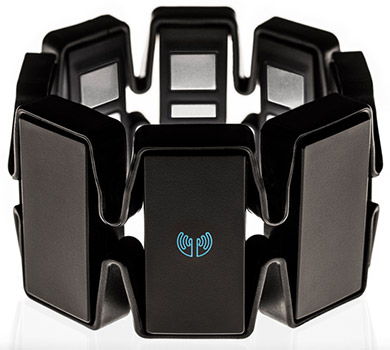
\includegraphics[height=5cm]{images/myoarmband.jpg}
    \captionsource{\url{https://s3.amazonaws.com/wordpressprod/blog/wp-content/uploads/2014/06/front-view.jpg}}
    \caption[The Myo Armband]{The Myo Armband}
    \label{fig:myoarmband}
\end{figure}


\section{Hardware}
The Myo armband consist of eight EMG sensors and nine-axis IMU containing gyroscope, accelerometer and magnetometer. The hardware specification is shown in \cref{table:myo_hardware}.

\begin{table}[ht!]
\centering
    \begin{tabular}{ | l | p{8cm} |}
        \hline
        \textbf{Sensors} & EMG sensor,\newline Gyroscope,\newline Accelerometer, \newline Magnetometer\\ \hline
        
        \textbf{Processor} & ARM Cortex M4 Processor  \\ \hline
        
        \textbf{Feedback} & Dual Indicator LEDs,\newline Short, Medium, Long Vibrations  \\ \hline
    \end{tabular}
    \caption[The Myo Hardware]{List of The Myo Hardware specifications}
    \label{table:myo_hardware}
\end{table}

\section{The Myo SDK}
\label{sec:myoSDK}
Thalmic Labs provides a SDK that allows developers to obtain access to the data from the Myo device. Since the Windows SDK was used, every statements in this report will be based on the Windows SDK.

The Myo armband provide applications with two type of data: Spatial data and gestural data.

\subsection{Spatial Data (IMU)}
Spatial data represents the location of the armband, and informs the applications about orientation and movements. This data is provided by the IMU. The Myo armband output three different data from the IMU: 
\begin{itemize}
  \item raw Accelerometer data
  \item raw Gyroscope data
  \item Orientation data
\end{itemize}
All which has a frame rate of 50 hz. Accelerometer data and gyroscope data is represented as 3D-vectors, with the unit g-force (accelerometer) and deg/s (gyroscope), while the orientation data from the magnetometer is represented as quaternions.

\subsection{Gestural Data (EMG sensor)}
Gestural data provide applications with information of less orientation depended movements, such as hand gestures. This data is provided by the EMG sensors. The Myo armband have eight EMG sensors, which outputs raw EMG data of 8-bit with a frame rate of 200 Hz \footnote{\url{http://developerblog.myo.com/raw-uncut-drops-today/}}. The MyoSDK documentation \cite{myoSDK} doesn't exactly provide information about the measurement unit, but the values are converted into a 8-bit value ranging from -128 to 128.
\chapter{Theory}
\label{chap:theory}

\section{Electomyography (EMG)}
Electromyography (EMG) is an electrodiagnostic medicine technique to measure muscle response or electrical activity produced by skeletal muscles \cite{wiki:Electromyography}. The nerves control the muscles by electrical signal called impulse, these impulses can be measured and analyzed \cite{WebMD:Electromyogram}. There are different method to measure those signals, but this project use surface EMG. Surface EMG is a technique where electrodes are places on the skin overlying a muscle to detect nerve impulses. 
\section{Inertial Measurement Unit (IMU)}
An inertial measurement unit (IMU) is an electronic device that measures linear and angular motion, usually with the combination of accelerometers and gyroscopes, but sometimes also with magnetometers. As described in \cref{chap:myo}, the Myo armband provide data from accelerometer, gyroscope and magnetometer.

\subsection{Gyroscope}
The gyroscope is used to measure or maintain the angular position. It consist of a disc (the rotor) that spins about an axis. Based on the principle of conservation of angular momentum, a spinning rotor will maintain it's orientation, thus the axis will be unaffected by tilts or rotations \cite{gyroscope_demonstration_project}. We can separate gyroscopes into three basic types:

\begin{itemize}
    \item Rotary (classical) Gyroscopes
    \item Vibrating Structure Gyroscopes
    \item Optical Gyroscopes
\end{itemize}

Since vibrating structure gyroscopes with MEMS technology are widely used in smart-phones and other electronic devices, we will take a closer look at vibrating structure gyroscopes \cite{vibrating_structure_gyroscope_wiki}. To better understand vibrating structure gyroscopes we need a basic understanding of the Coriolis effect. Every point on a rotating system will have the same angular velocity, but in order to travel a straight line towards or away from the axis of rotation, the traveling object have to either increase or decrease the linear velocity in order to maintain the relative angular position. The acceleration required to maintain the relative angular position is the Coriolis acceleration, an example is shown in \cref{fig:coriolis_acceleration} \cite{vibrating_structure_gyroscope}. Vibrating object tends to continue vibrating in the same plane even if its support rotates. The Coriolis effect causes the object to apply a force on its support, and by measuring this force the angular velocity can be determined \cite{vibrating_structure_gyroscope_wiki}.

\begin{figure}[ht]
    \centering
    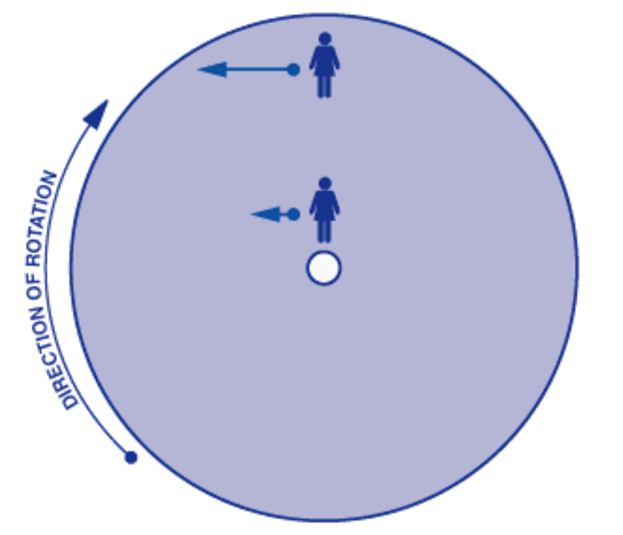
\includegraphics[height=5cm]{images/coriolis_acceleration.jpg}
    \captionsource{\url{http://www.analog.com/en/analog-dialogue/articles/imems-angular-rate-sensing-gyroscope.html}}
    \caption[Coriolis Acceleration Example]{A person trying to move northward toward the outer edge of a rotating platform. The linear velocity (Blue linear arrows) has to increase in order to maintain a northbound course. The acceleration is the Coriolis acceleration.}
    \label{fig:coriolis_acceleration}
\end{figure}


\subsection{Accelerometer}
An accelerometer is an electromechanical device to measure proper acceleration. Proper acceleration should not be confused with coordinate acceleration (rate of change of velocity). The measurement unit is given by g-forces ($g \approx 9.81m/s^{2}$), and by contrast to measuring coordinate acceleration, accelerometers in free fall will measure zero. 

There are many type of accelerometers, but to understand how the accelerometer work, we can use a simple model. Have in mind that this model is not exactly how a MEMS sensor work, but it explains the basic concept of accelerometers. To make this model simple, we will use a representation as shown in \cref{fig:accelerometer_model}. Imagine a ball inside a cube, when gravity pulls the ball down, it will hit at least one of the walls. The wall will according to Newton's third law have a force against the ball. This force is the measurement the accelerometer returns. This value can be represented by a vector \cite{IMU_guide}.

\begin{figure}[ht]
    \centering
    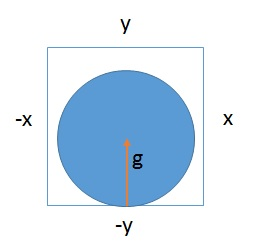
\includegraphics[height=5cm]{images/accelerometer.jpg}
    \caption[Accelerometer model]{2D representation model of a simple concept of an accelerometer. A ball is pushed down by gravity, and the accelerometer measure 1g at the -y wall.}
    \label{fig:accelerometer_model}
\end{figure}

\subsection{Magnetometer}
Magnetometer is a device that measure magnetic fields.
\section{Orientation Quaternions}
\label{sec:quaternion}
Euler Angles is one way to represent orientation, and it is based on that any orientation can be archived by rotations about the axes of a coordinate system. Compared to quaternions, Euler angles is simple and intuitive, but there are some ambiguities, one of those is the gimbal lock. In simple terms, gimbal lock is when two of the axis line up, and cause the rotating object to lose a degree of freedom. Quaternions introduce another approach to represent orientation that do not suffer from the gimbal lock, but is in return less intuitive and mathematically more complicated. This section will give a brief introduction to orientation quaternions, but we will not go into theoretical details on the quaternions. We will use the CH Robotics orientation sensors as the base of the descriptions \cite{CH_Robotics}.

The orientation quaternion can be estimated by rotation from the inertial frame to the body frame. The inertial frame is a fixed coordinate frame, such that the x-axis points north, the y-axes points east and the z-axis points in the gravitational direction. The body frame is a coordinate frame that is aligned with the sensor.

Quaternions are a number system that extends complex numbers, and is composed of one real element and three complex elements. It can be represented as a linear combination, such as
\begin{equation*}
    a + bi + cj + dk
\end{equation*}
where $a$, $b$,  $c$ and $d$ are real numbers, and $i$, $j$, and $k$ are the fundamental quaternion units. We can also represent quaternions as a four-element vector. Let the unit-vector quaternion rotation from the inertial frame to the body frame be defined as
\begin{equation*}
    \mathbf{q}^{b}_{i} = \begin{bmatrix}
            w \\
            x \\
            y \\
            z
        \end{bmatrix}
\end{equation*}

We can think of the elements $x$, $y$ and $z$ of the quaternion as a "vector part" that represent a vector about which rotation that should be performed, and that the element $w$ specifies the amount of rotation that should be performed about the vector part. Let $\theta$ be the angle of rotation and the vector $[v_x,v_y,v_z]^T$ be a unit vector representing the axis of rotation, then we can define the quaternion elements as

\begin{equation}
\label{eq:quaternion}
    \mathbf{q}^{b}_{i} = \begin{bmatrix}
            \cos{(\frac{1}{2}\theta)}\\
            v_x * \sin{(\frac{1}{2}\theta)}\\
            v_y * \sin{(\frac{1}{2}\theta)}\\
            v_z * \sin{(\frac{1}{2}\theta)}
        \end{bmatrix}
\end{equation}

In practice, we don't need to use this definition explicitly, but it provides an intuitive description of what the quaternion represents.
\section{Cross Correlation}
\label{sec:cross_correlation}
Cross Correlation is a method to estimate the degree of similarity of two series. Cross correlation works on any number of dimension, but for the purpose of this project, we only need to take a look at the one-dimensional cross correlation. Let $x$ and $y$ be two series, then we can define the one-dimensional normalized cross correlation $r$ at delay $d$ as	

\begin{equation}
\label{eq:cross_correlation}
    r(d) = \frac{\sum\limits_{i=0}\limits^{n} [(x(i) - \mean{x}) * (y(i-d) - \mean{y})]}{\sqrt{\sum\limits_{i=0}\limits^{n} (x(i) - \mean{x})^{2}} * \sqrt{\sum\limits_{i=0}\limits^{n} (y(i-d) - \mean{y})^{2}}},
\end{equation}

where $n$ is the number of point and $\mean{x}$ and $\mean{y}$ are the means of the corresponding series \cite{cross_correlation_theory}. The cross correlation have a range of -1 to 1. The value gives information about the series rises and falls relative to each other, where 0 indicating no correlation, $r > 0$ indicating positive correlation and  $r < 0$ indecating negativ correlation. If both rise at an identical rate, then we have $r = 1$, and opposite $r = -1$ if they fall at an identical rate. 

Given by the formula \ref{eq:cross_correlation} we get an issue when the index is less than 0 or when the index is greater than or equal to the number of points. The most common approach is to ignor this points and let $y(k) = 0$ if $k < 0$ or $k \geq n$ \cite{cross_correlation_code}.
\chapter{Methodology}
\chapter{Results}
\label{chap:results}
\chapter{Discussion}
\label{chap:discussion}

\section{Future Work}
\chapter{Conclusion}
\label{chap:conclusion}




% Bibliography - edit references.bib and use the \cite command in text
\renewcommand{\bibname}{References}
\bibliographystyle{plain}
\bibliography{references}
\clearpage

\pagenumbering{arabic}% resets `page` counter to 1
\renewcommand*{\thepage}{A-\arabic{page}}

\phantomsection
\addcontentsline{toc}{chapter}{Appendix}
\clearpage
\vspace*{\fill}
{\centering\huge\bfseries Appendix \par}
\vspace*{\fill}
\thispagestyle{empty}


\glsaddall % make it possible to print glossary without references
\printglossary[type=\acronymtype,title=Abbreviations, nonumberlist, style=super] % print the glossary
\addcontentsline{toc}{section}{Abbreviations}



\end{document}


